\section{Zielsetzung}
Bei diesem Versuch soll durch Ausnutzung der Interferenzbilder eines Einzelspalts
und zweier Doppelspalte deren Spaltbreite sowie gegebenenfalls der Abstand der
beiden Spalte bestimmt werden.



\section{Theorie}
\label{sec:Theorie}
\subsection{Fraunhofer Beugung}
Trifft Licht auf eine Öffnung bzw. ein Hinderniss, welches in etwa in der Größenordnung
der Wellenlänge liegt und zudem klein ist gegenüber dem Strahlendurchmesser, so kommt es zu
dem Phänomen der Beugung, welche sich durch die Welleneigenschaften des Lichtes erklären lässt.
Eine brauchbare Erklärung liefert das Huygenssche Prinzip der Elementarwellen, welches
besagt, dass sich von jedem Punkt einer Wellenfront eine kugelförmige Elementarwelle ausbreitet,
wobei sich diese Elementarwellen überlagen und konstruktiv oder destruktiv interferieren.


\noindent Bei der Beugung lassen sich im Allgemeinen zwei unterschiedliche Anordnungen
beschreiben, wobei bei diesem Versuch die Fraunhofersche verwendet wird.
Im Gegensatz zu der Fresnelschen liegt hier die Lichtquelle im Unendlichen (also praktisch:
sehr großer Abstand zwischen der Lichtquelle und dem Spalt im Vergleich zur Wellenlänge),
sodass die Wellenfront parallel auftrifft. Auch der Schirm befindet sich hierbei quasi im
Unendlichen, beispielsweise realisiert durch eine Sammellinse wie in Abbildung
\ref{fig:fraun}, sodass jeweils die Strahlen interferieren, welche unter dem gleichen
Winkel gebeugt wurden.

\begin{figure}[H]
  \centering
  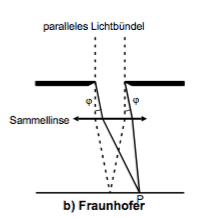
\includegraphics[height=7cm]{Fraunhofer.png}
  \caption{Fraunhofer Aufbau \cite{skript}.}
  \label{fig:fraun}
\end{figure}
\subsection{Einzelspalt}
Trifft nun zum Beispiel eine ebene Welle der Form
\begin{equation}
  A(z,t) = A_0 \exp{i(\omega t - 2\pi z / \lambda)}
  \label{eqn:welle}
\end{equation}
auf den Spalt, durchläuft sie diesen nicht nur gerade, sondern wird nach de bereits
erwähnten Huygensschen Prinzip hinter dem Spalt gebeugt, da sich die kugelförmigen
Elementarwellen in alle Richtungen ausbreiten.
Werden nun zwei Strahlenbündel betrachtet, welche an zwei unterschiedlichen Stellen
mit Abstand x auf den Spalt treffen und unter demselben Winkel $\phi$ gebeugt werden,
besitzen diese nach durchlaufen des Spaltes einen Wegunterschied s, aufgrund dessen
sich eine Phasendifferenz der Form
\begin{equation}
  \delta = \frac{2\pi \text{s}}{\lambda} = \frac{2\pi \text{x} \sin{\varphi}}{\lambda}
  \label{eqn:pdif}
\end{equation}
ergibt.
Die Gesamtwelle ergibt sich dabei durch Superposition der einzelnen Elementarwellen,
wegen des infinitesimalen Abstands dx der einzelnen Strahlenbündel geht die Summe
allerdings in eine Intergration über, wobei auch die bereits beschriebene Phasendifferenz
beachtet werden muss.
Es ergibt sich somit durch Umformung mit der Eulerschen Formel für den Sinus
folgende Formel für die Amplitude B unter dem Winkel $\varphi$ :
\begin{equation}
  B(z,t,\varphi) = A_0 \textbf{exp}\left\{i\left(\omega t - \frac{2\pi z}{\lambda}
  \right)\right\}\cdot \textbf{exp}\left\{\frac{\pi i b \sin{\varphi}}{\lambda}\right\} \cdot
  \frac{\lambda}{\pi \sin{\varphi}}\sin\left\{{\frac{\pi b \sin{\varphi}}{\lambda}}\right\}
  \label{eqn:einzel1}
\end{equation}
Diese Formel lässt sich durch die Substition
\begin{equation}
  \eta := \frac{\pi b \sin{\varphi}}{\lambda}
\end{equation}
zu
\begin{equation}
  B(\varphi) = A_0 b \frac{\sin{\eta}}{\eta}
  \label{eqn:einzel2}
\end{equation}
vereinfachen.
Eine solche Funktion ist in Abbildung \ref{fig:kurve} dargestellt.
\begin{figure}[H]
  \centering
  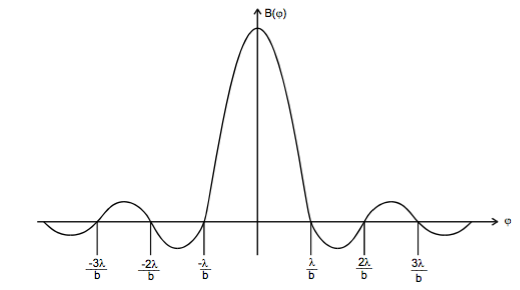
\includegraphics[height=7cm]{Kurve.png}
  \caption{B($\varphi$) einer ebenen Welle nach durchlaufen eines Einzelspalts \cite{skript}.}
  \label{fig:kurve}
\end{figure}
Da sich die Amplitude in der Praxis jedoch nicht direkt messen lässt, wird hier
die Intensität verwendet, welche durch die Funktion
\begin{equation}
  I(\varphi) \propto B(\varphi)^2 = A_0^2b^2\left(\frac{\lambda}{\pi b \sin{\varphi}}\right)^2
  \cdot \sin^2\left\{{\frac{\pi b sin{\varphi}}{\lambda}}\right\}
  \label{eqn:int1}
\end{equation}
\subsection{Doppelspalt}
\begin{figure}[H]
  \centering
  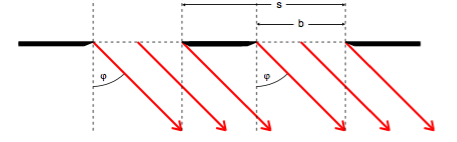
\includegraphics[height=3cm]{Doppel.png}
  \caption{Beugung am Doppelspalt \cite{skript}.}
  \label{fig:doppel}
\end{figure}
Zur Berechnung des Beugungsmusters eines Doppelspalts, wird dieser als
Überlagerung der Beugungsbilder zweier einzelner Spalte betrachtet, sodass
sich eine Intensitätsverteilung von
\begin{equation}
  I(\varphi) \propto B(\varphi)^2 =4 \cdot \cos^2\left\{{\frac{\pi s \sin{\varphi}}{\lambda}}\right\}
  \cdot \left(\frac{\lambda}{\pi b \sin{\varphi}}\right)^2 \cdot \sin^2\left\{{\frac{\pi
  b \sin{\varphi}}{\lambda}}\right\}
  \label{eqn:doppelinf}
\end{equation}
erbibt, wobei s den Abstand der Spalte beschreibt und b die Breite, wie in Abbildung
\ref{fig:doppel} zu sehen ist.
